\chapter{Contents of the CD disk}
The included CD disk contains:
\begin{itemize}
\item
Source codes of two NLG systems used in the experiment of Chapter \ref{chap:exper}
\item
Data collected in the experiment of Chapter \ref{chap:exper}
\item
Electronic version of this thesis
\end{itemize}


The source codes of Alpha and Beta NLG systems are in a format of Apache Maven project and should be therefore easily compiled. The data from the experiment are in the GIVE log format, stored in CSV format.

\chapter{Histograms for first reference machine learning}
This chapter contains attributes' histograms for timing of the first reference ML.
\begin{figure}[!htbp]
  \centering
	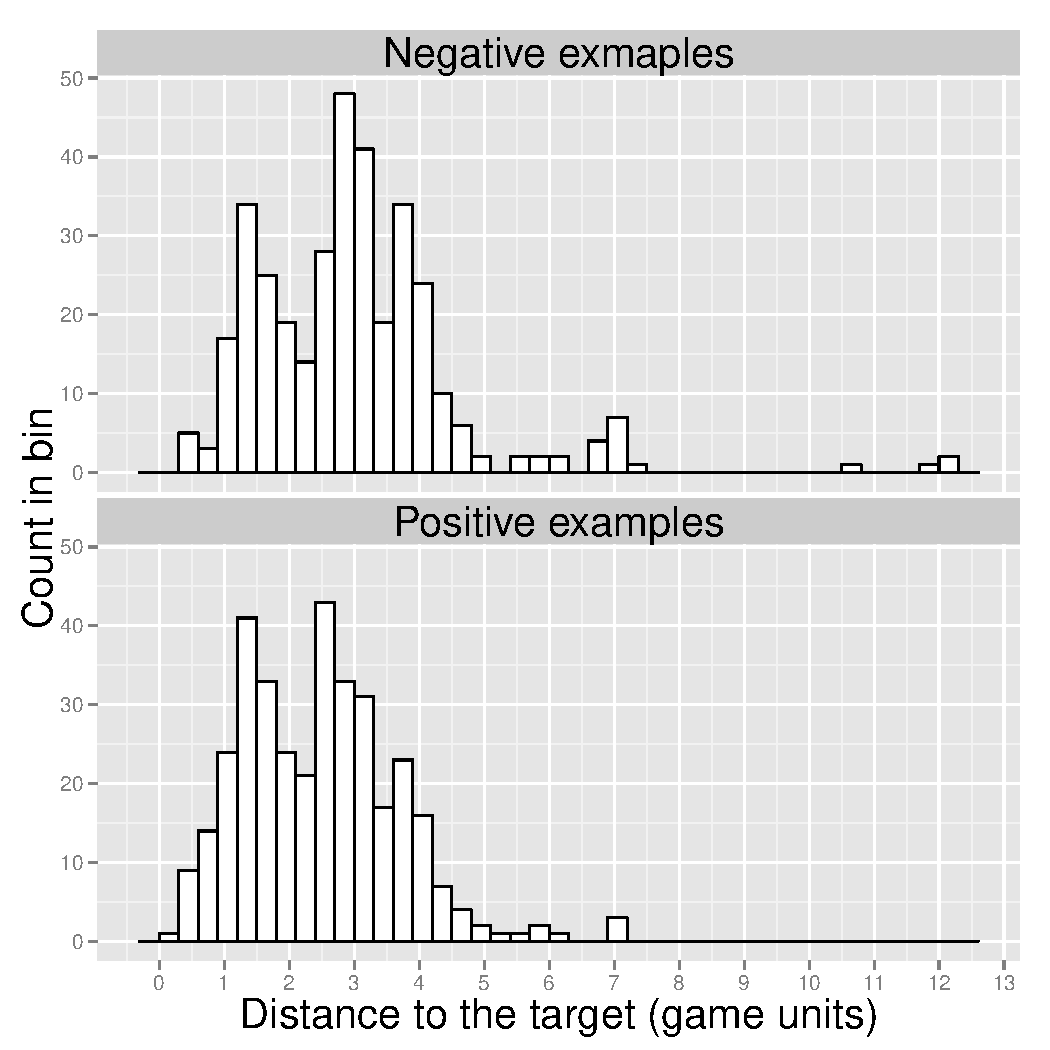
\includegraphics[page=1,width=0.6\textwidth]{Images/fref_distrib}
	\caption{Histogram of attribute distance to the target}
	\label{fig:fref-distrib-dist}
\end{figure}

\begin{figure}[!htbp]
  \centering
	\includegraphics[page=2,width=0.6\textwidth]{Images/fref_distrib}
	\caption{Histogram of attribute angle to the target}
	\label{fig:fref-distrib-angle}
\end{figure}

\begin{figure}[!htbp]
  \centering
	\includegraphics[page=3,width=0.6\textwidth]{Images/fref_distrib}
	\caption{Histogram of attribute whether the target is visible}
	\label{fig:fref-distrib-visib}
\end{figure}

\begin{figure}[!htbp]
  \centering
	\includegraphics[page=4,width=0.6\textwidth]{Images/fref_distrib}
	\caption{Histogram of attribute number of distractors}
	\label{fig:fref-distrib-distractors}
\end{figure}

\begin{figure}[!htbp]
  \centering
	\includegraphics[page=5,width=0.6\textwidth]{Images/fref_distrib}
	\caption{Histogram of attribute number of distracting buttons}
	\label{fig:fref-distrib-distbuttons}
\end{figure}

\begin{figure}[!htbp]
  \centering
	\includegraphics[page=6,width=0.6\textwidth]{Images/fref_distrib}
	\caption{Histogram of attribute number of distracting buttons with lesser angle}
	\label{fig:fref-distrib-distangles}
\end{figure}

\FloatBarrier

\chapter{Histograms for chains machine learning}
This chapter contains attributes' histograms for chains ML.
\begin{figure}[!htbp]
  \centering
	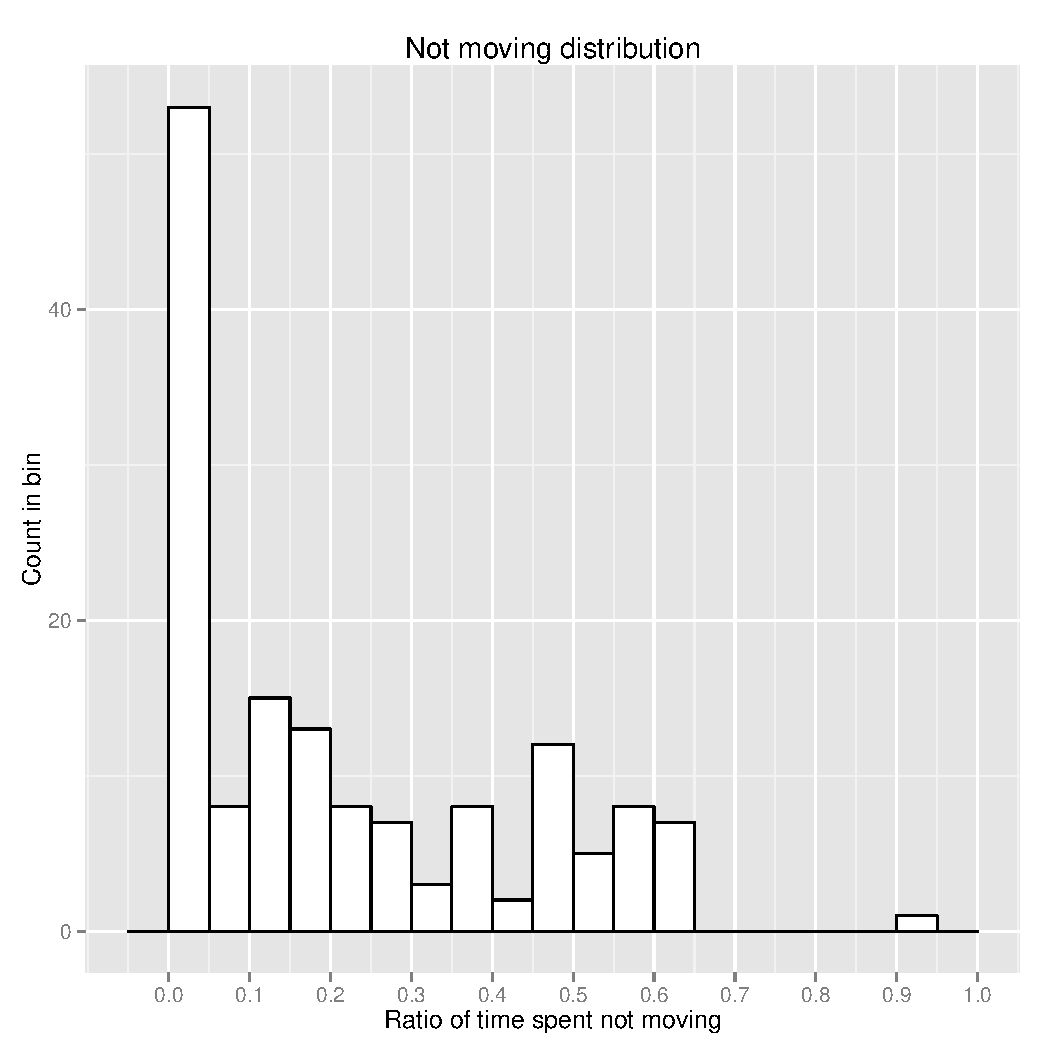
\includegraphics[page=1,width=0.6\textwidth]{Images/chains_features_ML}
	\caption{Histogram of attribute time spent not moving}
	\label{fig:chains-distrib-stop}
\end{figure}

\begin{figure}[!htbp]
  \centering
	\includegraphics[page=2,width=0.6\textwidth]{Images/chains_features_ML}
	\caption{Histogram of attribute time spent rotating}
	\label{fig:chains-distrib-rotate}
\end{figure}

\begin{figure}[!htbp]
  \centering
	\includegraphics[page=3,width=0.6\textwidth]{Images/chains_features_ML}
	\caption{Histogram of attribute objects in the room}
	\label{fig:chains-distrib-objects}
\end{figure}

\begin{figure}[!htbp]
  \centering
	\includegraphics[page=4,width=0.6\textwidth]{Images/chains_features_ML}
	\caption{Histogram of attribute buttons in the room}
	\label{fig:chains-distrib-buttons}
\end{figure}

\begin{figure}[!htbp]
  \centering
	\includegraphics[page=5,width=0.6\textwidth]{Images/chains_features_ML}
	\caption{Histogram of attribute landmarks in the room}
	\label{fig:chains-distrib-landmarks}
\end{figure}

\begin{figure}[!htbp]
  \centering
	\includegraphics[page=6,width=0.6\textwidth]{Images/chains_features_ML}
	\caption{Histogram of attribute very close buttons to the target}
	\label{fig:chains-distrib-veryclose}
\end{figure}

\begin{figure}[!htbp]
  \centering
	\includegraphics[page=7,width=0.6\textwidth]{Images/chains_features_ML}
	\caption{Histogram of attribute buttons on the same wall as the target}
	\label{fig:chains-distrib-samewall}
\end{figure}

\begin{figure}[!htbp]
  \centering
	\includegraphics[page=8,width=0.6\textwidth]{Images/chains_features_ML}
	\caption{Histogram of attribute close buttons to the target}
	\label{fig:chains-distrib-close}
\end{figure}

\begin{figure}[!htbp]
  \centering
	\includegraphics[page=9,width=0.6\textwidth]{Images/chains_features_ML}
	\caption{Histogram of attribute far buttons from the target}
	\label{fig:chains-distrib-far}
\end{figure}